\clearpage
\section*{Appendix}
%%%%%%%%%%%%%%%%%%%%%%%%%%%%%%%%%%%%%%%%%%%%%%%%%%%%
% Verification of the Constructed Marginal Velocity
%%%%%%%%%%%%%%%%%%%%%%%%%%%%%%%%%%%%%%%%%%%%%%%%%%%%
\section{Verification of the Constructed Marginal Velocity}\label{app:continuity}

Under our construction $x_t = (1-t) x_0 + t z$, the trajectory of each sample is deterministic and given by a simple affine transformation. Such deterministic transform preserves the total probability mass: the density is only shifted and rescaled. Consequently, the evolution of $p_t(x_t \mid z)$ must satisfy the continuity equation:
%
\begin{equation*}
\frac{\partial}{\partial} p_t(x_t \mid z) + \nabla_{x_t} \cdot (p_t(x_t \mid z) \cdot v(x_t, t \mid z)) = 0.
\end{equation*}
%
Consider the marginal probability density:
%
\begin{align*}
\frac{\partial}{\partial t} p_t(x_t) &= \frac{\partial}{\partial t} \int p_t(x_t \mid z) p_\text{target}(z) dz \\
&= \int  \frac{\partial}{\partial t} p_t(x_t \mid z) p_\text{target} (z) dz.
\end{align*}
%
Substitute $\dfrac{\partial}{\partial t} p_t(x_t \mid z)$ with the continuity equation:
%
\begin{align*}
\frac{\partial}{\partial t} p_t(x_t)
&= \int - \nabla_{x_t} \left( p_t(x_t \mid z) \cdot v(x_t, t \mid z) \right) p_\text{target} (z) \, dz \\
&= - \nabla_{x_t} \cdot \int v(x_t, t \mid z) \cdot p_t(x_t \mid z) p_\text{target} (z) \, dz \\
&= - \nabla_{x_t} \cdot \int v(x_t, t \mid z) \frac{p_t(x_t \mid z) p_\text{target}(z)}{p_t (x_t)} p_t(x_t) dz \\
&= - \nabla_{x_t} \cdot \left( \left( \int v(x_t, t \mid z) \frac{p_t(x \mid z) p_\text{target}(z)}{p_t (x_t)} dz \right) \cdot p_t(x_t) \right) \\
&= - \nabla_{x_t} \cdot \left( v^\text{tgt}(x_t, t) \cdot p_t(x_t) \right).
\end{align*}

%%%%%%%%%%%%%%%%%%%%%%%%%%%%%%%%%%%%%%%%%%%%%%%%%%%%
% Conclusion of the Linear-Form Error
%%%%%%%%%%%%%%%%%%%%%%%%%%%%%%%%%%%%%%%%%%%%%%%%%%%%
\section{Conclusion of the Linear-Form Error}\label{app:linear_func}
We show that whenever the error term is a linear function of the target velocity $v^\text{tgt}(x_t,t)$, the same training gradient can be obtained by substituting it with the conditional velocity $v(x_t,t \mid z)$.
%
Formally, assume
\begin{equation*}
\text{error} = A v^\text{tgt}(x_t, t) - b_\theta,
\end{equation*}
%
where $A$ is a matrix independent of the learnable parameters $\theta$, and $b_\theta$ is a function of $\theta$.


Define the marginal and conditional loss function as:
%
\begin{align}
  \mathcal{L_\text{marginal}} &= \mathbb{E}_{t, x_t \sim p_t} \left[ \left\| b_\theta - A v^\text{tgt} (x_t, t) \right\|_2^2 \right] \\
  \mathcal{L_\text{conditional}} &=  \mathbb{E}_{t, z \sim p_\text{target}, x_t \sim p_t(\cdot \mid z)} \left[ \left\| b_\theta - A v (x_t, t \mid z) \right\|_2^2 \right]
\end{align}
%
The expectations of $\|b_\theta\|_2^2$ under both measures coincide.
%
Besides, $\left\| A v^\text{tgt} (x_t, t) \right\|_2^2$ and $\left\| A v (x_t, t \mid z) \right\|_2^2$ are independent of $\theta$.
%
And we show that:
%
\begin{align*}
\mathbb{E}_{t, x_t \sim p_t} \left[ b_\theta^\top A v^\text{tgt}(x_t, t) \right] &= \iint b_\theta^\top A v^\text{tgt}(x_t, t) p_t(x_t) \, dt \, dx_t \\
&= \iint b_\theta^\top A \left( \int v(x_t, t \mid z) \frac{p_t(x_t \mid z) p_\text{target}(z)}{p_t(x_t)} \, dz \right) p_t(x_t) \, dt \, dx_t \\
&= \iiint b_\theta^\top A v(x_t, t \mid z) p_t(x_t \mid z) p_\text{target}(z) \, dz \, dt \, dx_t \\
&= \mathbb{E}_{t, z \sim p_\text{target}, x_t \sim p_t(\cdot \mid z)} \left[ b_\theta^\top A v(x_t, t \mid z) \right]
\end{align*}

This shows that $\mathcal{L}_\text{marginal}$ and $\mathcal{L}_\text{conditional}$ yield identical gradients with respect to $\theta$ whenever the error depends linearly on $v^\text{tgt}(x_t,t)$.

%%%%%%%%%%%%%%%%%%%%%%%%%%%%%%%%%%%%%%%%%%%%%%%%%%%%
% Conclusion of the Linear-Form Error
%%%%%%%%%%%%%%%%%%%%%%%%%%%%%%%%%%%%%%%%%%%%%%%%%%%%
\section{MeanFlow with Classifier-Free Guidance}\label{app:cfg}

We extend MeanFlow with classifier-free guidance (CFG) by modifying the marginal velocity field. Specifically, the CFG-enhanced marginal velocity is defined as:
\begin{equation*}
  v_\text{cfg} (x_r, r \mid c) = \omega v(x_r, r \mid c) + (1 - \omega) u(x_r, r, r),
\end{equation*}
where $c$ denotes the conditioning label, and $u(x_r, r, r)$ denotes the unguided instantaneous marginal velocity.  Since there's no closed-form of $u(x_r, r, t)$, we use a neural network approximation $u^\theta_\text{cfg}(x_r, r, t)$, leading to:
%
\begin{equation}
  v_\text{cfg} (x_r, r \mid c) = \omega v(x_r, r \mid c) + (1 - \omega) u^\theta_\text{cfg} (x_r, r, r).
\end{equation}
%
Substituting $v^\text{tgt}(x_r, r)$ in Equation~\eqref{mf_basic_eq} with $v_\text{cfg}(x_r, r \mid c)$, we derive the target CFG average velocity field to train $u^\theta_\text{cfg}(x_r, r, t \mid c)$:
\begin{equation}\label{eq:cfg_marginal}
  u_\text{cfg}^\text{tgt} (x_r, r, t) = v_\text{cfg} (x_r, r \mid c) + (t - r) \left( \frac{\partial u^\theta_\text{cfg}}{\partial x_r} v_\text{cfg}(x_r, r \mid c) + \frac{\partial u^\theta_\text{cfg}}{\partial r} \right)
\end{equation}

The error term $u^\theta_\text{cfg}(x_r, r, t) - u^\text{tgt}_\text{cfg}(x_r, r, t)$ is linear with respect to the marginal velocity $v(x_r, r \mid c)$. Following conclusion in Appendix~\ref{app:linear_func}, we replace the marginal velocity $v_\text{cfg}(x_r, r \mid c)$ in Equation~\eqref{eq:cfg_marginal} with the conditional CFG velocity $v_\text{cfg}(x_r, r \mid c, z)$. Since $v(x_r, r \mid c, z) = v(x_r, r \mid z) = z - x$, the conditional CFG velocity becomes:
%
\begin{align}
  v_\text{cfg} (x_r, r \mid c, z) &= \omega v(x_r, r \mid c, z) + (1 - \omega) u_\text{cfg}^\theta(x_r, r, r) \nonumber \\
  &= \omega v(x_r, r \mid z) + (1 - \omega) u_\text{cfg}^\theta(x_r, r, r),
\end{align}
%
This leads to the final results in Equation~\eqref{mf_cfg_tgt} and Equation~\eqref{v_cond_cfg}.


%%%%%%%%%%%%%%%%%%%%%%%%%%%%%%%%%%%%%%%%%%%%%%%%%%%%
% Learning Rate and Loss
%%%%%%%%%%%%%%%%%%%%%%%%%%%%%%%%%%%%%%%%%%%%%%%%%%%%
\section{Learning Rate and Loss During Training}\label{app:rate_and_loss}

\vspace{1cm}
\begin{minipage}[c]{\linewidth}
  \centering
  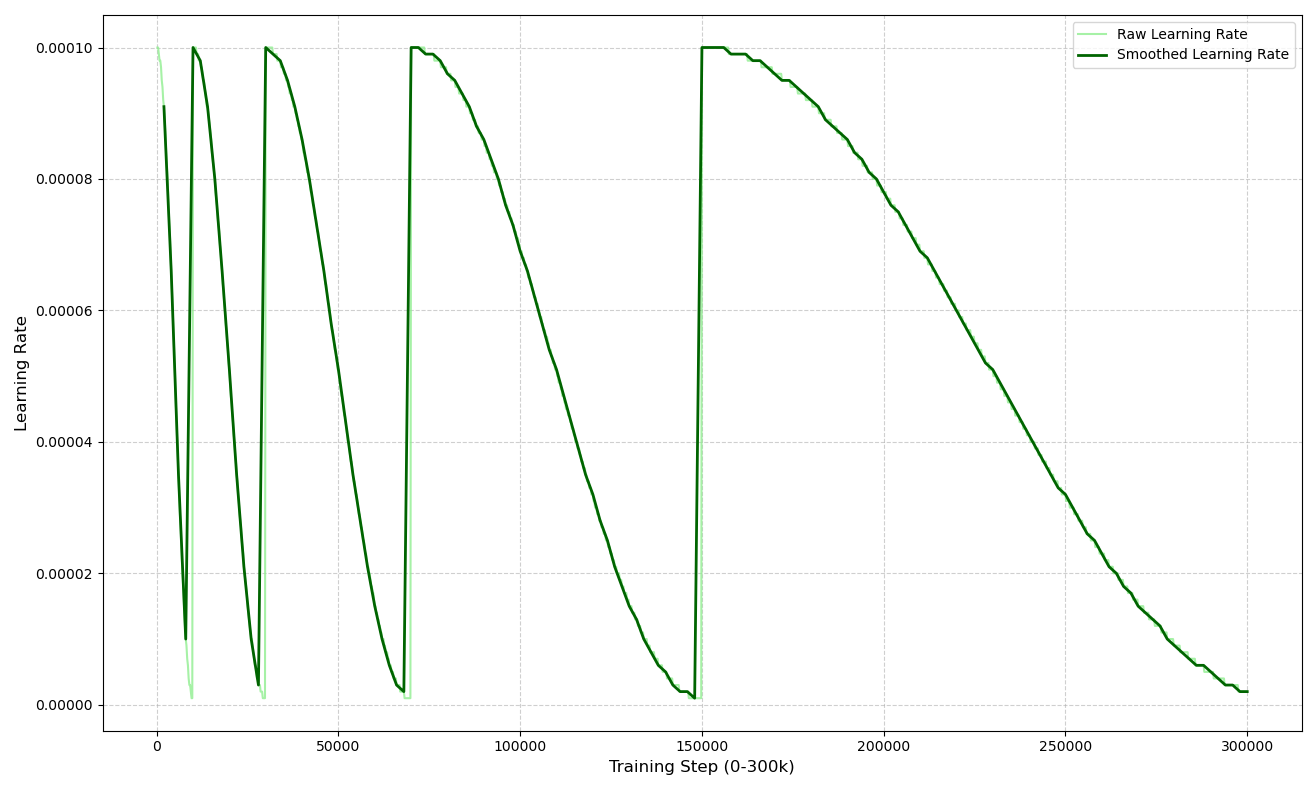
\includegraphics[width=0.9\linewidth]{figures/learning_rate.png}
  \captionof{figure}{Learning rate over training.}
\end{minipage}
\vspace{1cm}
\begin{minipage}[c]{\linewidth}
  \centering
  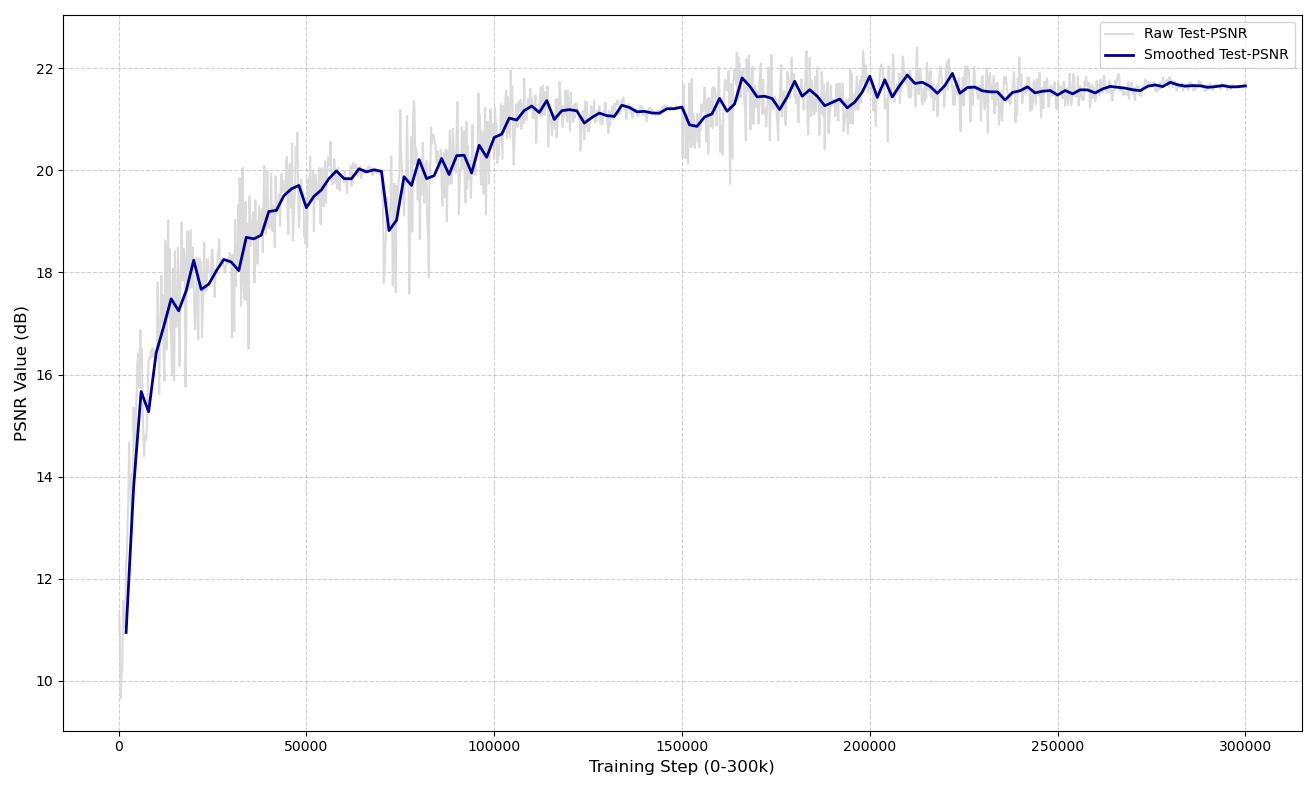
\includegraphics[width=0.9\linewidth]{figures/psnr_over_step.png}
  \captionof{figure}{Loss and MSE loss over training.}
\end{minipage}
\vspace{1cm}
